\documentclass[12pt]{article}
\usepackage{graphicx,multicol}
\title{Generative Adverserial Network}
\author{Harshal Patel\\2019pcp5048 MNIT Jaipur}
\date{October, 2019}

\begin{document}
\maketitle

\section*{Abstract}
Earlier neural networks are only used for classification , regression and object detection only but using generative neural network computer can generate artificial images,music,etc. Aim of this paper\cite{GAN} is to provide an basic information about what genrative adverserial network is and where they are used.


\section{Introduction}
In generative neural network instead of training only one neural network, we are training two neural networks one for generating artifical images and one for detecting whether image came from original input set or from generator.It is like minimax game. Purpose of Generator is to maximize probability of Descriminator making mistake.
It can be seen as counterfeiters, trying to make fake currency and cop trying to detect it.
Generator and descriminator are trained using multilayer perceptron by backpropogation .




\section{Applications}
GANs are trained on wide range of datasets from MNIST, toronto face detection , and CIFAR.
Generator network uses linear and sigmoid activation functions while descriminator uses maxout activation. dropout technique is used to remove neurons in order to avoid overfitting. 


\begin{center}


\begin{table}
\begin{tabular}{ c | c | c } 
 \hline
Model & MNIST & TFD\\
 \hline
 DBN & 138±2 & 1909±66\\

Deep GSN & 121±1.6 & 2110±50\\
Adverserial Nets & 225±2 & 2017±26


\end{tabular}
\caption{Parzen window-based log-likelihood estimates. The reported numbers on MNIST are the mean loglikelihood of samples on test set, with the standard error of the mean computed across examples}
\end{table}
\end{center}


\begin{figure}
\centering
\begin{minipage}{.45\textwidth}
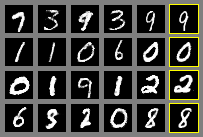
\includegraphics[width=\textwidth]{mnist1.png}
\caption{image generated from mnist dataset}
\end{minipage}
~~~~
\begin{minipage}{.45\textwidth}
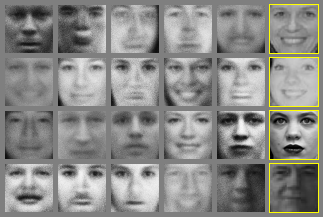
\includegraphics[width=\textwidth]{tfd1.png}
\caption{image generated from TFD dataset}
\end{minipage}
\end{figure}


\section{Types of GAN}
\subsection{Vanilla GAN}
This is the simplest type of GAN\cite{GAN} and in this case the generator and the discriminator are just simple multi-layer perceptrons. Vanilla GANs simply just seek to optimize the mathematical equation using stochastic gradient descent
\subsection{DCGAN}
DCGAN(deep convolution GAN)\cite{ImageNet} is one of the most popular types of GANs\cite{GAN} today. In this case, ConvNets are used in place of the multi-layer perceptrons. The objective function remains the same here. 
\subsection{Progressive GAN}

Progressive Gan is the progressive growing of GAN. The GAN\cite{GAN} is trained multiple times. It is mainly used for high resolution image generation.
In phase 1, it takes in a latent feature z and uses two convolution layers to generate 4×4 images. Then, we train the discriminator with the generated images and the 4×4 real images. Once the training stables, we add 2 more convolution layers to upsampling the image to 8×8 and 2 more convolution layers to down sampling images in the discriminator.
\subsection{SRGAN}
image super resolution can be defined as increasing size of image and keeping minimum drop in quality of image, keeping minor details of image. This problem is quite complex than it seems.\\
Our main target is to reconstruct super resolution image or high resolution image by up-scaling low resolution image such that texture detail in the reconstructed SR images is not lost.\\
There are various ways of enhancing image quality. One of the most commonly used technique is interpolation. This is easy to use but this leads to distorted image or reduces the visual quality of image. Most common interpolation methods produce blurry images, i.e. bi-cubic interpolation.
In training Generator network dropout method is used in order to avoid overfitting. 

\begin{figure}[hbt!]
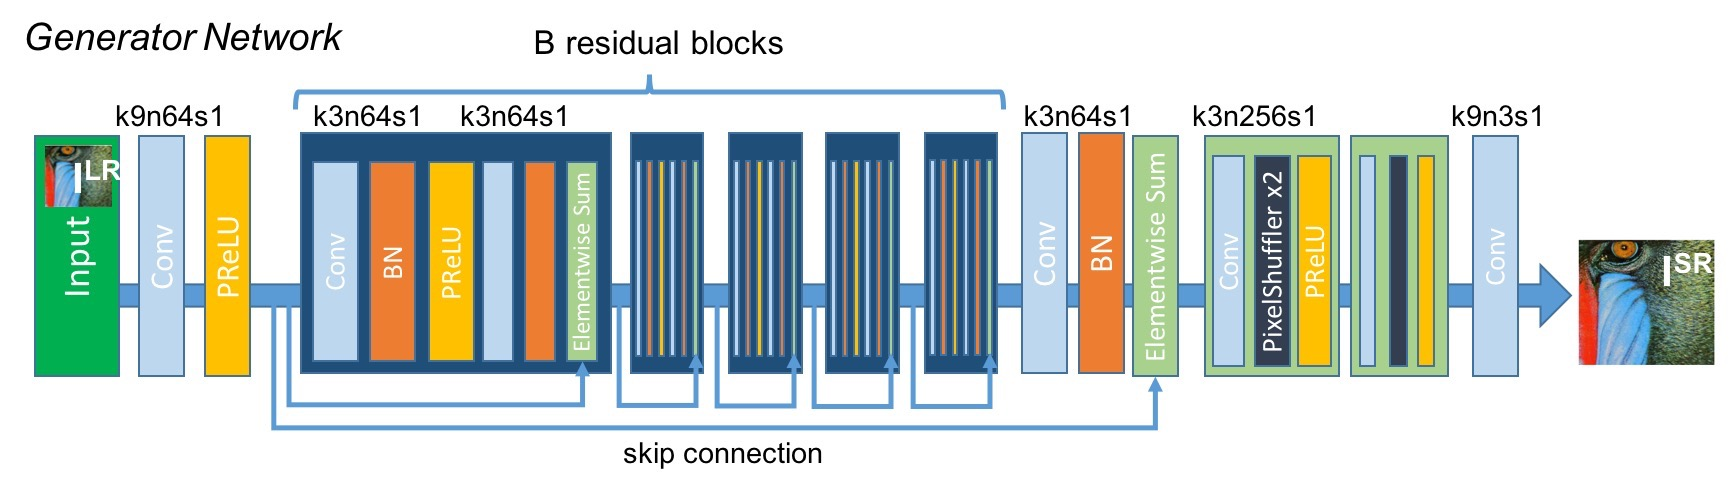
\includegraphics[scale=0.39]{srgang.png}
\caption{SRGAN Generator architecture}\end{figure}\begin{figure}
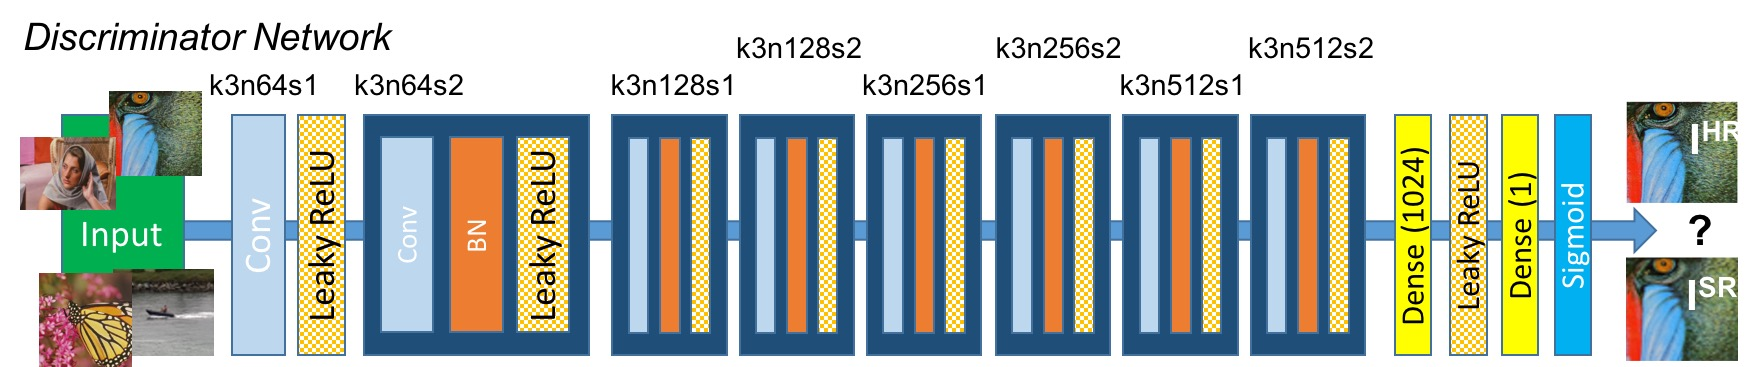
\includegraphics[scale=0.39]{srgand.png}
\caption{SRGAN descriminator architecture}
\end{figure}
%\clearpage




\begin{thebibliography}{9}

\bibitem{GAN}
Ian J. Goodfellow et al.,
"Generative Adversarial Nets",
2014,


\bibitem{SRGAN}
Christian Ledig et al.,
"Photo-Realistic Single Image Super-Resolution Using a Generative Adversarial
Network",
May 2017,
\ref{}
\bibitem{CNN}
Jayanth Koushik,
"Understanding Convolutional Neural Networks",
2016,
\bibitem{ImageNet}
Alex Krizhevsky et al.,
"ImageNet Classification with Deep Convolutional
Neural Networks"

\end{thebibliography}
\end{document}


\end{document}